\documentclass[12pt]{article}
\usepackage{amsfonts, epsfig}

\usepackage{graphicx}
\usepackage{fancyhdr}
\pagestyle{fancy}
\lfoot{\texttt{github.com/conorhoughton/COMS30127}}
\lhead{Computation Neuroscience - 4\_numberical (b) - Conor}
\rhead{\thepage}
\cfoot{}
\begin{document}

\section*{Numerical integration of differntial equations} 

This lecture is about the Taylor series and about the numerical
solution of differential equations; two methods are considered, the
Euler method and the Runge Kutta method. These are the most
straight-forward way to solve differential equations on a computer,
there are other methods that are commonly used in neuroscience, like
backwards Runge Kutte and adaptive timestep methods, but these are
easy enough to understand in the future once you know about Euler and
Runge Kutta.

\subsection*{The Taylor series}

As an introduction it is often useful to use a series description of
functions, it can help with numerical calculations of the values and
it can be useful in studying properties of the function. Here, it will
be used to work out how to efficiently calculate the solutions to
differential equations accurately. The Taylor series is one commonly
applicable approach to representing a function as a series.

Imagine you have a function $f(t)$ that can be represented as a series
\begin{equation}
f(t)=\sum_{n=0}^\infty{a_nt^n}=a_0+a_1t+a_2t^2+\ldots
\end{equation}
Now, putting $t=0$ we get
\begin{equation}
f(0)=a_0
\end{equation}
Next, differentiate
\begin{equation}
\frac{df(t)}{dt}=a_1+2a_2t+3a_3t^2+\ldots=\sum_{n=1}^\infty{a_nnt^{n-1}}
\end{equation}
so, putting $t=0$ we get
\begin{equation}
\frac{df}{dt}|_{t=0}=a_1
\end{equation}
Differentiating again gives
\begin{equation}
\frac{d^2f(t)}{dt^2}=2a_2+6a_3t+12a_4t^2\ldots=\sum_{n=1}^\infty{a_nn(n-1)t^{n-2}}
\end{equation}
so
\begin{equation}
\frac{1}{2}\frac{d^2f}{dt^2}|_{t=0}=a_2
\end{equation}
and so on.

In fact, by this sort of calculation we see that
\begin{equation}
a_n=\frac{1}{n!}\left.\frac{d^nf}{dt^n}\right|_{t=0}
\end{equation}
or, put another way, 
\begin{equation}
f(t)=\sum_{n=0}^\infty\frac{1}{n!}\left.\frac{d^nf}{dt^n}\right|_{t=0}t^n
\end{equation}
This is the Taylor series. We haven't proven that $f(t)$ has a series
of the form $\sum_{n=0}^\infty a_nt^n$ at all and not all functions
do, in particular, if the function is badly behaved at $t=0$ it may
not. We also haven't proved that the series converges. If we write
\begin{equation}
f(t)=\sum_{n=0}^{N-1}\frac{1}{n!}\left.\frac{d^nf}{dt^n}\right|_{t=0}t^n+E_N(t)
\end{equation}
where $E_N(t)$ represents the error from stopping at after $N$ terms,
we might expect $E_N(t)$ vanishes as $N$ goes to infinity. In fact,
this doesn't always happen and sometimes, even when the series does
converge, it does so very slowly, so $E_N(t)$ remains large even for
very large values of $N$. Frequently the series converges for some
values of $t$ but not for others. Nonetheless, the Taylor series is
often useful.

You might already know the series expansion of $\exp{t}$, but lets
calculate it as a Taylor series. Since
\begin{equation}
\frac{d}{dt}\exp{t}=\exp{t}
\end{equation}
we know
\begin{equation}
\frac{d^n}{dt^n}\exp{t}=\exp{t}
\end{equation}
or
\begin{equation}
\left.\frac{d^n}{dt^n}\exp{t}\right|_{t=0}=1
\end{equation}
for all $n$ so
\begin{equation}
f(t)=\sum_{n=0}^{\infty}\frac{1}{n!}t^n
\end{equation}
which is what we got before.

Next lets consider
\begin{equation}
f(t)=\sin{t}
\end{equation}
Now 
\begin{equation}
\frac{d}{dt}f(t)=\cos{t}
\end{equation}
and
\begin{equation}
\frac{d^2}{dt^2}f(t)=-\sin{t}
\end{equation}
and so on. Putting $t=0$ and using $\sin{0}=0$ and $\cos{0}=1$ we get
\begin{equation}
\sin{t}=\sum_{n\,\mbox{odd}}\frac{(-1)^{(n-1)/2}t^n}{n!}
\end{equation}

Finally, we have been expanding around $t=0$, but you can expand around any point, here we expand around $t=t_0$
\begin{equation}
f(t)=\sum_{n=0}^\infty\frac{1}{n!}\left.\frac{d^nf}{dt^n}\right|_{t=t_0}(t-t_0)^n
\end{equation}
or, writing $\epsilon=t-t_0$
\begin{equation}
f(t_0+\epsilon)=\sum_{n=0}^\infty\frac{1}{n!}\left.\frac{d^nf}{dt^n}\right|_{t=t_0}\epsilon^n
\end{equation}

\subsection*{Numerical solutions of differential equations}

Consider the differential equation
\begin{equation}
\frac{df}{dt}=G(f)
\end{equation}
This class of differential equations would include the equation we looked before:
\begin{equation}
\frac{df}{dt}=-\frac{1}{\tau}f
\end{equation}
with $G(f)=-f/\tau$. Of course, the right hand side might also depend
on $t$, but we'll worry about that later. Imagine we want to find
numerical values for $f(t)$ where we know $f(0)=f_0$, some value, and
\begin{equation}
\frac{df}{dt}=G(f)
\end{equation}
Imagine further that we can't solve the equation analytically, so we
resort to solving it approximately on the computer. This might be
necessary because the equation is too hard to solve, or, in the case of the equation
\begin{equation}
\tau\frac{df}{dt}=g(t)-f(t)
\end{equation}
it might be that we don't know $g(t)$ analytically.

The normal approach would be to discretize time and to work out the
solution approximately for each time step in turn, depending on the
previous time step. In other words, say we choose $\delta t$, a small
value, as the time step then we would work out $y(\delta t)$, then use
that to work out $y(2\delta t)$ and so on.

Let us use the notation $f_n=f(n\delta t)$ and consider how we might
get a computer to work out $f_{n+1}$ approximately if $f_n$ is already
known. Now, by the Taylor expansion
\begin{equation}
f(n\delta t+\delta t)=f(n\delta
t)+\left.\frac{df}{dt}\right|_{t=n\delta t}\delta
t+\frac{1}{2}\left.\frac{d^2f}{dt^2}\right|_{t=n\delta t}(\delta t)^2+\ldots
\end{equation}
so one simple approach is to ignore the $(\delta t)^2$ and smaller terms, since $df/dt=G(f)$ this gives
\begin{equation}
f_{n+1}=f_n+G(f_n)\delta t
\end{equation}
This approximation is known as the \textsl{Euler method}. A simple example is plotted in Fig.~1.

\begin{figure}
\begin{center}
  \setlength{\unitlength}{0.0500bp}%
  \begin{picture}(5040.00,3528.00)%
      \put(946,1087){\makebox(0,0)[r]{\strut{} 2.5}}%
      \put(946,1725){\makebox(0,0)[r]{\strut{} 5}}%
      \put(946,2363){\makebox(0,0)[r]{\strut{} 7.5}}%
      \put(946,3002){\makebox(0,0)[r]{\strut{} 10}}%
      \put(1078,484){\makebox(0,0){\strut{} 0}}%
      \put(1821,484){\makebox(0,0){\strut{} 1}}%
      \put(2563,484){\makebox(0,0){\strut{} 2}}%
      \put(3306,484){\makebox(0,0){\strut{} 3}}%
      \put(4049,484){\makebox(0,0){\strut{} 4}}%
      \put(176,1983){\rotatebox{-270}{\makebox(0,0){\strut{}$f$}}}%
      \put(2860,154){\makebox(0,0){\strut{}$t$}}%
      \put(3656,1097){\makebox(0,0)[r]{\strut{}euler}}%
      \put(3656,877){\makebox(0,0)[r]{\strut{}$\exp(0.5t)$}}%
    \put(0,0){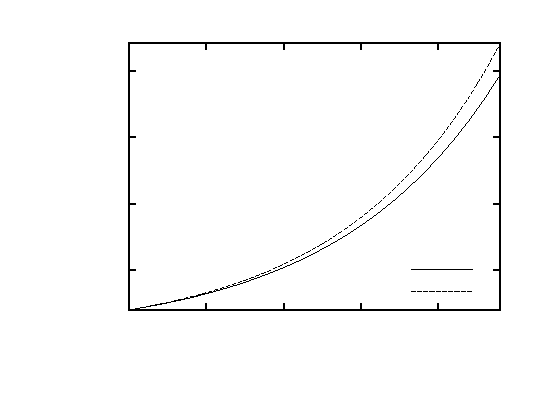
\includegraphics{euler_approx}}%
  \end{picture}%


\end{center}
\caption{A comparison of the Euler method with the true solution for
  the equation $df/dt=rf$ with $r=0.5$. This equation in actually one where
  the Euler method works quite well for modest values of $t$, here a
  large time step of $\delta t=0.2$ is used to emphasise the error,
  the actual solution is plotted for
  comparison.}
\end{figure}

\subsection*{The Runge-Kutta method}

The Runge-Kutta method uses the Taylor expansion in a clever way to
find a better approximation than the Euler mdthod. It is a bit
convoluted, so there is a lot of notation, but it does give a very
useful numerical algorithm.

As before, we want to solve
\begin{equation}
\frac{df}{dt}=G(f)
\end{equation}
with a time discretization of $\delta t$, $f_n$ is the approximate
value the algorithm calculates for $f(n\delta t)$ and $f_0=f(0)$, the
initial condition. Now say we are at $f_n$ and let
\begin{equation}
k_1=G(f_n)
\end{equation}
so the Euler approximation would be $f_{n+1}=f_n+k_1\delta t$. Next, let
\begin{equation}
k_2=G\left(f_n+\frac{\delta t k_1}{2}\right)
\end{equation}
Now, using the Taylor expansion
\begin{equation}
k_2=G(f_n+\delta t f_1/2)=G(f_n)+\left.\frac{dG}{df}\right|_{f=f_n}\delta t\frac{k_1}{2}+\ldots
\end{equation}
Substituting back for $k_1$ this gives
\begin{equation}
k_2=G(f_n)+\frac{1}{2}\left.\frac{dG}{dg}\right|_{g=g_n}\left.\frac{dg}{dt}\right|_{t=t_n}\delta t+\ldots
\end{equation}
Using the chain rule
\begin{equation}
\frac{d^2g}{dt^2}=\frac{dG}{dt}=\frac{dG}{df}\frac{df}{dt}
\end{equation}
so
\begin{equation}
k_2=G(y_n)+\frac{1}{2}\frac{d^2f}{dt^2}\delta t+\ldots
\end{equation}
Now, recall
\begin{equation}
f(n\delta t + \delta t)=f_n+\left.\frac{df}{dt}\right|_{t=t_n}\delta t+\frac{1}{2}\left.\frac{d^2f}{dt^2}\right|_{t=t_n}\delta t^2+\ldots
\end{equation}
and from the formula for $k_1$ and $k_2$ we see that this can be written as
\begin{equation}
y_{n+1}=y_n+k_2\delta t
\end{equation}
This means that the calculation of $y_{n+1}$ takes into account of
more of the Taylor expansion that the Euler method, it includes the
$\delta t^2$ part and so the errors will come in at $\delta t^3$.
This is the \textsl{second order Runge Kutta method}, it is called
second order because it include the first and second order terms in
the Taylor expansion, the Euler method is like a first order Runge
Kutta method.

The second order Runge Kutta method isn't usually used; it is the
fourth order Runge Kutta that is considered the standard way of doing
numerical integration. The idea is just the same as the one we saw
above, by combining different terms more of the Taylor expansion is
accounted for, in fact, as the name suggests, the fourth order Runge
Kutta gets everything up to the fourth order, the errors are like
$\delta t^5$.

Here I will give the fourth order Runge Kutta and will include the
possibility that the right hand side of the differential equation also
includes a dependence on $t$ so, writing $t_n=n\delta t$
\begin{equation}
\frac{df}{dt}=G(t,f)
\end{equation}
Now
\begin{eqnarray}
k_1&=&G(t_n,f_n)\cr
k_2&=&G\left(t_n+\frac{1}{2}\delta,f_n+\frac{1}{2}\delta tk_1\right)\cr 
k_3&=&G\left(t_n+\frac{1}{2}\delta,f_n+\frac{1}{2}\delta tk_2\right)\cr 
k_4&=&G\left(t_n+\delta,y_n+\delta tk_2\right) 
\end{eqnarray}
and 
\begin{equation}
f_{n+1}=f_n+\frac{1}{6}(k_1+2k_2+2k_3+k_4)
\end{equation}

\begin{figure}
\begin{center}
% GNUPLOT: LaTeX picture with Postscript
\begingroup
  \makeatletter
  \providecommand\color[2][]{%
    \GenericError{(gnuplot) \space\space\space\@spaces}{%
      Package color not loaded in conjunction with
      terminal option `colourtext'%
    }{See the gnuplot documentation for explanation.%
    }{Either use 'blacktext' in gnuplot or load the package
      color.sty in LaTeX.}%
    \renewcommand\color[2][]{}%
  }%
  \providecommand\includegraphics[2][]{%
    \GenericError{(gnuplot) \space\space\space\@spaces}{%
      Package graphicx or graphics not loaded%
    }{See the gnuplot documentation for explanation.%
    }{The gnuplot epslatex terminal needs graphicx.sty or graphics.sty.}%
    \renewcommand\includegraphics[2][]{}%
  }%
  \providecommand\rotatebox[2]{#2}%
  \@ifundefined{ifGPcolor}{%
    \newif\ifGPcolor
    \GPcolorfalse
  }{}%
  \@ifundefined{ifGPblacktext}{%
    \newif\ifGPblacktext
    \GPblacktexttrue
  }{}%
  % define a \g@addto@macro without @ in the name:
  \let\gplgaddtomacro\g@addto@macro
  % define empty templates for all commands taking text:
  \gdef\gplbacktext{}%
  \gdef\gplfronttext{}%
  \makeatother
  \ifGPblacktext
    % no textcolor at all
    \def\colorrgb#1{}%
    \def\colorgray#1{}%
  \else
    % gray or color?
    \ifGPcolor
      \def\colorrgb#1{\color[rgb]{#1}}%
      \def\colorgray#1{\color[gray]{#1}}%
      \expandafter\def\csname LTw\endcsname{\color{white}}%
      \expandafter\def\csname LTb\endcsname{\color{black}}%
      \expandafter\def\csname LTa\endcsname{\color{black}}%
      \expandafter\def\csname LT0\endcsname{\color[rgb]{1,0,0}}%
      \expandafter\def\csname LT1\endcsname{\color[rgb]{0,1,0}}%
      \expandafter\def\csname LT2\endcsname{\color[rgb]{0,0,1}}%
      \expandafter\def\csname LT3\endcsname{\color[rgb]{1,0,1}}%
      \expandafter\def\csname LT4\endcsname{\color[rgb]{0,1,1}}%
      \expandafter\def\csname LT5\endcsname{\color[rgb]{1,1,0}}%
      \expandafter\def\csname LT6\endcsname{\color[rgb]{0,0,0}}%
      \expandafter\def\csname LT7\endcsname{\color[rgb]{1,0.3,0}}%
      \expandafter\def\csname LT8\endcsname{\color[rgb]{0.5,0.5,0.5}}%
    \else
      % gray
      \def\colorrgb#1{\color{black}}%
      \def\colorgray#1{\color[gray]{#1}}%
      \expandafter\def\csname LTw\endcsname{\color{white}}%
      \expandafter\def\csname LTb\endcsname{\color{black}}%
      \expandafter\def\csname LTa\endcsname{\color{black}}%
      \expandafter\def\csname LT0\endcsname{\color{black}}%
      \expandafter\def\csname LT1\endcsname{\color{black}}%
      \expandafter\def\csname LT2\endcsname{\color{black}}%
      \expandafter\def\csname LT3\endcsname{\color{black}}%
      \expandafter\def\csname LT4\endcsname{\color{black}}%
      \expandafter\def\csname LT5\endcsname{\color{black}}%
      \expandafter\def\csname LT6\endcsname{\color{black}}%
      \expandafter\def\csname LT7\endcsname{\color{black}}%
      \expandafter\def\csname LT8\endcsname{\color{black}}%
    \fi
  \fi
  \setlength{\unitlength}{0.0500bp}%
  \begin{picture}(5040.00,3528.00)%
    \gplgaddtomacro\gplbacktext{%
      \csname LTb\endcsname%
      \put(946,1087){\makebox(0,0)[r]{\strut{} 2.5}}%
      \put(946,1725){\makebox(0,0)[r]{\strut{} 5}}%
      \put(946,2363){\makebox(0,0)[r]{\strut{} 7.5}}%
      \put(946,3002){\makebox(0,0)[r]{\strut{} 10}}%
      \put(1078,484){\makebox(0,0){\strut{} 0}}%
      \put(1821,484){\makebox(0,0){\strut{} 1}}%
      \put(2563,484){\makebox(0,0){\strut{} 2}}%
      \put(3306,484){\makebox(0,0){\strut{} 3}}%
      \put(4049,484){\makebox(0,0){\strut{} 4}}%
      \put(176,1983){\rotatebox{-270}{\makebox(0,0){\strut{}$f$}}}%
      \put(2860,154){\makebox(0,0){\strut{}$t$}}%
    }%
    \gplgaddtomacro\gplfronttext{%
      \csname LTb\endcsname%
      \put(3656,1097){\makebox(0,0)[r]{\strut{}rk}}%
      \csname LTb\endcsname%
      \put(3656,877){\makebox(0,0)[r]{\strut{}$\exp(0.5t)$}}%
    }%
    \gplbacktext
    \put(0,0){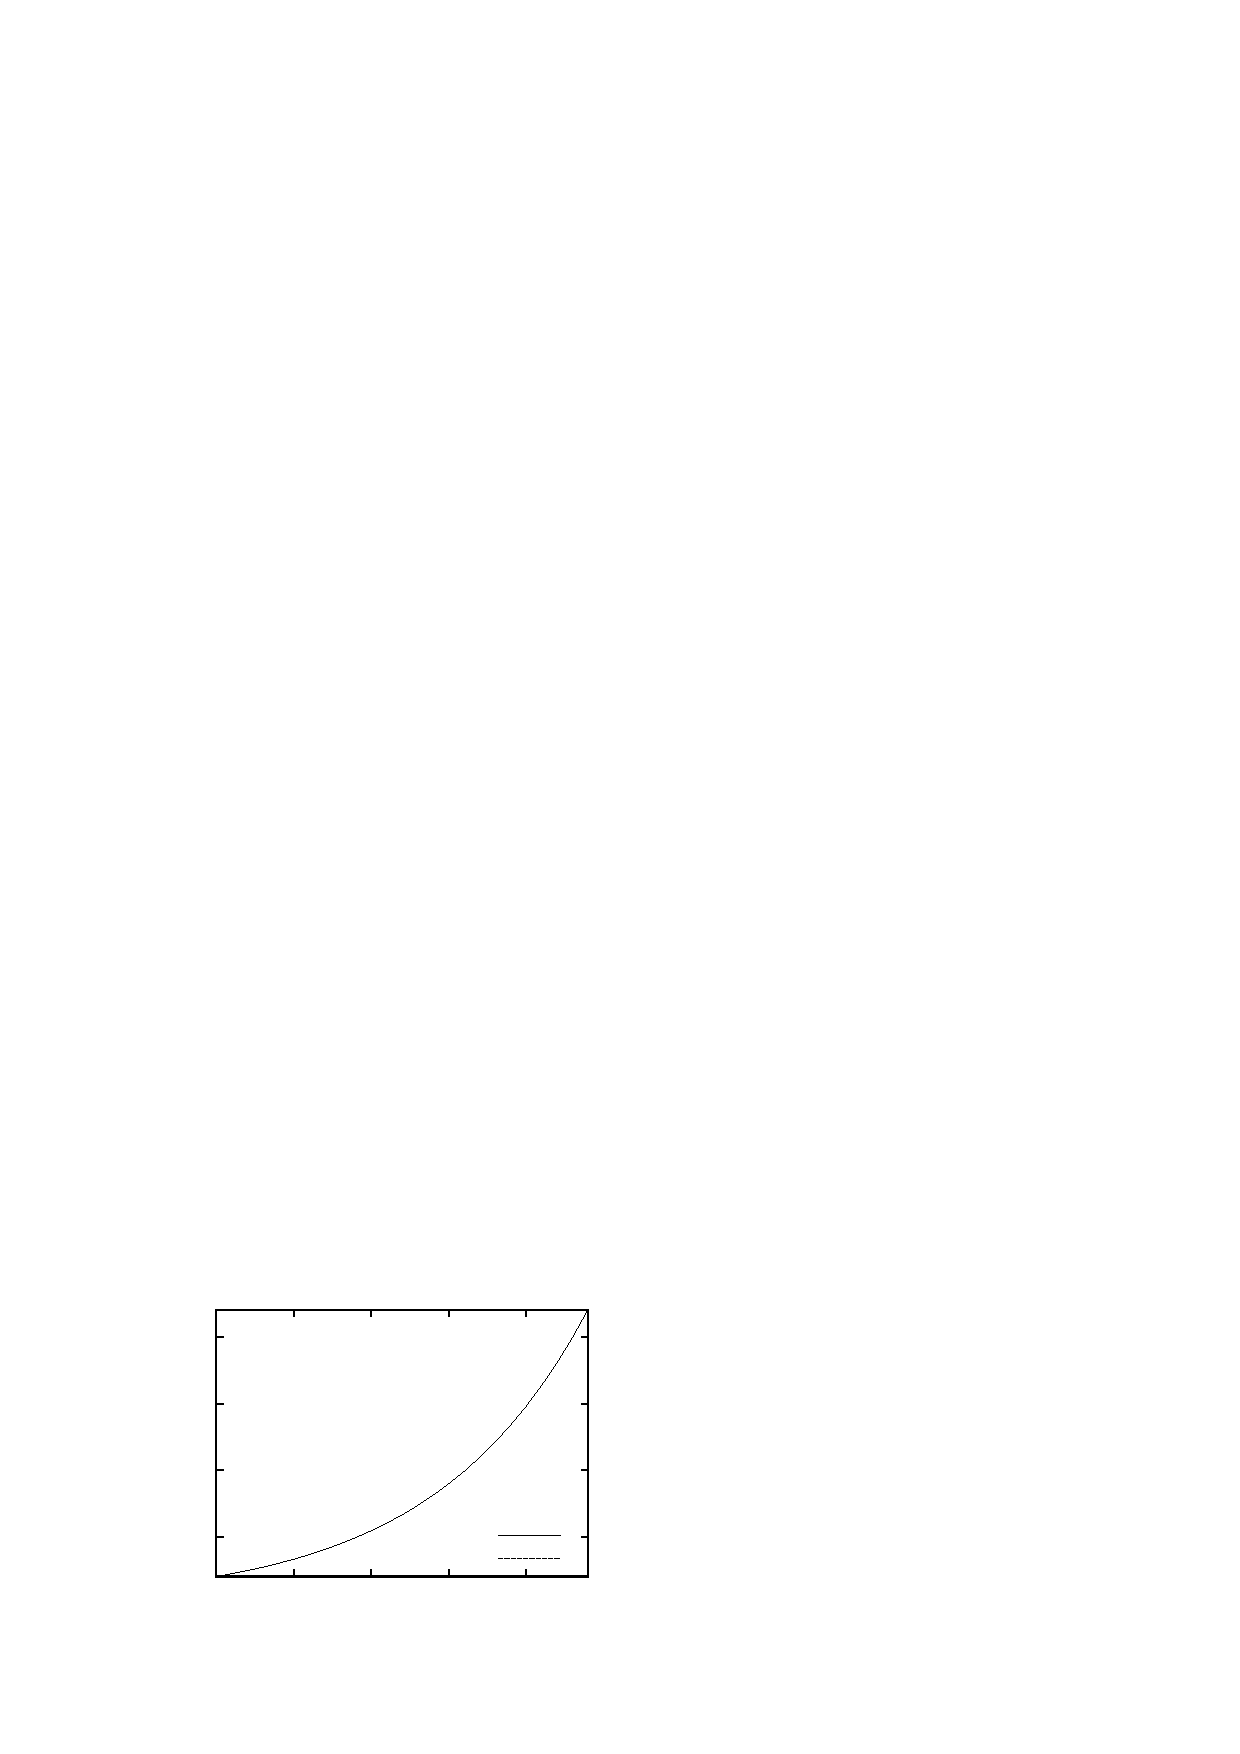
\includegraphics{rk_approx}}%
    \gplfronttext
  \end{picture}%
\endgroup

\end{center}
\caption{A comparison of the fourth order Runge Kutta method with the
  true solution for the growth equation. This has the same values of
  $r$ and $\delta t$ as in Fig.~1, but the fourth order Runge-Kutta
  method is used instead of the Euler method. As you can see, the
  approximation and true solution are indistinguishable.}
\end{figure}


\end{document}

